\documentclass[10pt,preprint,onecolumn]{article}
\usepackage[utf8]{inputenc}
\usepackage[spanish]{babel}
\usepackage[T1]{fontenc}
\usepackage{mathtools, comment, url, hyperref}
\usepackage[cm]{fullpage}
\usepackage{setspace}
\usepackage{float}
\usepackage{wrapfig}
\usepackage[pdftex]{graphicx}
\usepackage{tikz}
\usetikzlibrary{trees}
\usepackage{caption}
\usepackage{cite}
\usepackage{subcaption}
\usepackage{lscape}
\restylefloat{figure}
\singlespacing

\begin{document}

%% proceso de extraccion, limitaciones fisicas, logicas, movilidad
%% no gps, priorizacion, alertas, nodos heterogeneos

Para determinar la comunicación existente y posible en minería, es necesario separar la minería de rajo abierto, que suele contar con redes celulares negociadas directamente con los proveedores de internet  ---exceptuando aquellas de pequeña escala y artesanal---, y la minería subterránea, donde no existen los medios de comunicación disponibles en la superficie. Por esto, ha surgido tecnología dedicada a la minería subterránea, que a su vez cuenta con una gran variabilidad de ambientes como túneles y galerías. A continuación se presenta una revisión de las características más importantes en estos ambientes, tomadas del estudio realizado por Mauricio Contreras \cite{tesis} de comunicación en minas chilenas subterráneas, y del informe interno de Codelco para Intraestructura en Minas Subterráneas\cite{doccodelco}.

\section{Características Importantes}

La comunicación en minería es fundamental para la coordinación de actividades, imprescindible para evitar accidentes que pueden ser fatales. Se hace énfasis a la comunicación de seguridad, tanto de datos tomados por sensores como de alertas para notificar un potencial problema humano que podría desencadenar una falla de mayor escala.

\begin{enumerate}
\item \textbf{Robustez:} Dado que las minas subterráneas están sujetas a potenciales colapsos y otros riesgos, la habilidad de un equipo de comunicación de emergencia de mantenerse operacional ante un accidente es fundamental. Por ello, se requiere una infraestructura de red que no se desconecte con un daño estructural.

\item \textbf{Flexibilidad:} El ambiente de las minas está continuamente cambiando por el proceso de extracción. Esto resulta en una necesidad continua de expandir y modificar la conectividad necesaria. Los sistemas que requieren un gran esfuerzo de instalación ofrecen una menor flexibilidad, pero a la vez, un sistema totalmente inalámbrico puede congestionarse al expandirse el sistema.

\item \textbf{Rango/Cobertura:} Dadas las distancias potencialmente largas entre los operarios, y el hecho de que la topología de la mina es complicada y cambiante, es necesaria una alta cobertura en las distintas ubicaciones donde puedan estar desarrollándose las actividades. Los sistemas de radio, ampliamente utilizados en minería, poseen un alcance bajo al estar bajo tierra.
\end{enumerate}

\section{Comunicación actual}
En la actualidad, existen topologías de red principalmente cableadas en minas subterráneas, especialmente en aquellas donde la operación es guiada remotamente, por lo que se requiere una conectividad en tiempo real para obtener un desempeño óptimo. Aún así, existen diversas zonas y niveles de varios kms de longitud donde no existe conectividad más allá de las radios portadas por equipos de operarios.

Existe un espectro de frecuencias (entre 600 y 3000Hz) que permite una propagación de señal de radio a distancias considerables a través de la tierra (\emph{Through the Earth} o TTE), pero requieren la instalación de antenas muy grandes, por lo que necesitan un espacio grande para ser instaladas. Estas suelen brindar comunicación en una dirección, usando una antena grande en el exterior y equipos pequeños sobre los operarios, que pueden recibir información en caso de emergencias tal como las áreas afectadas o las rutas de escape.

El uso de radios entre operarios es basado en Push-To-Talk (PTT), donde los operarios deben sintonizar un mismo canal, y presionar un botón para hablar, y luego soltándolo para escuchar. Las radios usualmente permiten varios canales, pudiendo sincronizar grupos a través del uso de éstos. 

Es también común dividir a los usuarios, desde una perspectiva de comunicación, por sus unidades jerárquicas (como mantenimiento, operaciones, supervisores, etc). Una unidad jerárquica puede poseer uno o más canales asignados. Cabe mencionar que las distintas unidades conviven en los mismos espacios, pero el alto ruido ambiental y las orejeras utilizadas por ello hacen que no fluya información entre los distintos grupos.

Estos factores generan segregación de operarios en grupos pequeños (al alcance de radio) y divididos por jerarquías, que sólo obtienen información desde el exterior, sin poder notificar el estado actual de la zona entre sí ni hacia el exterior.
\part*{Requerimientos}
Antes de comparar protocolos, resulta interesante analizar cuáles son las hipótesis de la red sobre la que queremos trabajar.
Primero, consideraremos que existen dos tipos de tráfico:

\begin{enumerate}
    \item Alarmas, sensibles al delay y de alta prioridad, pero de volumen pequeño
    \item Monitoreo, tolerante al delay y de baja prioridad, pero de gran volumen.
\end{enumerate}

Nuestra prioridad consiste, primero, en entregar una solución del menor delay y mayor tasa de recepción de paquetes al primer caso, y hacer el mejor esfuerzo para el segundo. 

Una hipótesis de las DTN es que no se conoce la topología y evolución de la red, por lo que sólo podemos intentar predecir las mejores rutas y esperar que eventualmente existan. En nuestro formato, tendremos un pequeño conocimiento de la red, dado por los roles específicos que juegan los operarios en las minas, a pesar de las distintas topologías que éstas tengan. A continuación se listan algunas hipótesis que repercutirán en la decisión de enrutamiento:

\begin{enumerate}
    \item Existen distintas categorías de operarios, puesto que cada uno tiene una labor específica en la mina.
    \item Los operarios se mantienen durante su jornada en una zona acotada a su rubro específico. Estas zonas pueden ser muy grandes, sobre todo si trabaja con equipo móvil como camionetas o camiones.
    \item Existen supervisores que viajan entre las distintas zonas para verificar las operaciones, convirtiéndose en nodos que unen áreas posiblemente desconectadas.
    \item Existen diversos equipos que pueden utilizarse para mejorar la entrega de mensajes: camiones, grúas y camionetas se desplazan de manera constante a través de las minas, tanto de rajo abierto como subterráneas. También existe maquinaria específica de las áreas, que puede utilizarse como almacenamiento y fuetne de energía, pero cuya conectividad es limitada. 
    \item Diariamente los operarios deben pasar por zonas específicas como los casinos, donde se puede garantizar que entre cualquier par de operarios de la misma categoría existirá un camino, pero usarlo para enrutar puede aportar mucho delay (horas).
\end{enumerate}

Estos factores nos permiten inferir algunos datos del movimiento esperados y de la evolución de la topología de la red, lo cual se debe considerar a la hora de realizar simulaciones y, en particular, de definir los patrones de movimiento para los distintos nodos, los cuales afectan directamente el desempeño de los protocolos.

Primero, se espera que los operarios que \emph{conectan} distintas áreas, a saber, supervisores y operarios sobre equipo móvil, sean nodos de mayor prioridad en enrutamiento hacia otras áreas, al tener una mayor probabilidad de viajar entre ellas.
También, se cuenta con un peor caso para el monitoreo donde los datos se descarguen al final del día. Esto puede no ser factible si la duración de la batería y almacenamiento no es suficiente para los datos de todo el día.

\begin{comment}
\newpage

\part*{Taxonomía de Protocolos para DTN}

\newpage
\begin{landscape}

\begin{figure}[H]
\begin{tikzpicture}
  [auto,every node/.style={rectangle,draw, text centered, text width=2.0cm,minimum height=1.5cm },node distance=4cm]
\tikzset{%
level 1/.style={sibling distance = 11.1cm, level distance=2cm,edge from parent path={(\tikzparentnode.south) -- (\tikzchildnode.north)}},
level 2/.style={sibling distance = 7.5cm, level distance=2cm,edge from parent path={(\tikzparentnode.south) -- (\tikzchildnode.north)}},
level 3/.style={sibling distance = 2.5cm, level distance=2cm,edge from parent path={(\tikzparentnode.south) -- (\tikzchildnode.north)}},
level 4/.style={sibling distance = 2.5cm, level distance=2cm,edge from parent path={(\tikzparentnode.south) -- (\tikzchildnode.north)}},
level 5/.style={sibling distance = 2.5cm, level distance=2cm,edge from parent path={(\tikzparentnode.south) -- (\tikzchildnode.north)}},
level 6/.style={sibling distance = 2.5cm, level distance=2cm,edge from parent path={(\tikzparentnode.south) -- (\tikzchildnode.north)}},
}

\node (0){DTN}
    child {node (1) {Replicativo}
              child {node (2) {Replicativo \\Controlado}
                child{node (3) {Sin Info \\ adicional}
                    child[blue]{node (4) {Spray and \\Wait}}}
                child{node {Función de \\ utilidad}
                    child[blue]{node {Spray and Focus}
                    child{node {SCAR}
                    child{node {CRHC}}}}}
                child{node {Historia de \\ encuentros}
                    child[blue]{node{PRoPHET}}}
                child{node {Estimación \\ probabilista}
                    child[blue]{node{Plankton}}}}
              child {node {Replicativo \\Ilimitado}
                child{node {Sin Info \\ adicional}
                    child[blue]{node {Epidemic}}}
                child{node {Estimación \\ probabilista}
                    child[blue]{node {MaxProp}
                    child{node {RAPID}}}}}
              }
    child {node {Forwarding}
              child {node (5){Historia de \\ encuentros}
                child[blue] {node (6){PER}
                child {node {SMART}}}}
              child {node (5){Información \\ social}
                child[blue] {node (6){SOLAR}
                child {node {BUBBLE}}}}};
\end{tikzpicture}

\end{figure}

\end{landscape}
\newpage
 A continuación se presenta una taxonomía para algunos protocolos de DTN representativos, cubriendo una gran porción de las estrategias utilizadas en estas redes. Todos los protocolos buscan maximizar la probabilidad de entrega, para lo cual utilizan diferentes datos para estimar los vínculos que existirán y la posibilidad de utilizarlos en la entrega de mensajes. 
 
\section{Replicativos}
Se realizan copias de los mensajes para entregarlos a otros nodos, que se enrutan al mismo tiempo hacia el mismo destino. El número de copias puede ser fijo, mediante configuración del protocolo, o bien entrenarse según avance la transmisión de datos.

Las copias generadas pueden ser o bien \emph{controladas}, donde el protocolo genera una candidad acotada de copias, buscando aumentar la probabilidad de entrega sin saturar la red de mensajes idénticos; o bien \emph{ilimitadas}, donde se realizan nuevas copias siempre que resulte conveniente, sin tomar en consideración el número actual de copias.

\subsection{Replicativo controlado}
Dentro de las copias controladas, existe una diversidad de mecanismos para definir cómo controlar estas copias tomando en cuenta distinta información del entorno. Esta información en general toma en cuenta la historia de encuentros entre nodos ---surgiendo a la vez el problema de cómo obtener o estimar esta información--- buscando maximizar la probabilidad de entrega con ello. 

%epidemic limitado, entrega directa
\subsubsection{Spray-and-Wait}
Spray-and-Wait\cite{sandw} es un protocolo que realiza forward y entrega directa, en dos fases distintas. El nodo de origen genera L copias, que esparce según cierta distribución. Normalmente se utiliza spray binario, es decir, cada nodo reparte la mitad de sus copias al nodo que encuentra, esperando que éste a su vez entregue la mitad al topar un nuevo nodo que no tenga el mensaje, como se ve en la Figura \ref{fig:hpa}; o spray directo, donde sólo el nodo de origen reparte 1 copia a cada nodo que ve. Al terminar el spray, es decir, cuando cada nodo cuenta con sólo una copia, si no se encontró al destinatario en esa fase, se pasa a esperar, donde cada nodo intenta entregar el mensaje directamente al nodo final.
Spray-and-Wait obtiene mejores resultados que los protocolos de \emph{flooding}.

\begin{figure}[h]
\centering
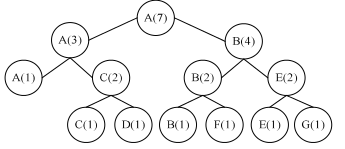
\includegraphics[width=200px]{HPA.png}
\caption{Spray Binario \cite{crhc}}
\label{fig:hpa}
\end{figure}

%epidemic limitado, funcion de utilidad
\subsubsection{Spray-and-Focus}
Spray-and-Focus\cite{sandf} es una variante posterior de Spray-and-Wait, donde una vez esparcidas las $L$ copias no se alcanza el destinatario sólo mediante entrega directa. Cuando un nodo encuentra a un mejor candidato, entrega su copia a éste, espandiendo así las posibilidades de llegar al destiantario. El problema de esta estrategia es que incorpora la optimización de cierta función de utilidad para determinar cuándo reenviar, erradicando la simpleza inherente a Spray and Wait, y no teniendo la mejora suficiente para justificarlo. Aún así, resulta novedoso incorporar la idea de mejorar la inteligencia durante la segunda fase.

%orientado a sensores-sink, tipo spray-and-focus con R copias, utility function
\subsubsection{SCAR}
El protocolo SCAR\cite{scar}, orientado a sensores de baja independencia energética, busca tomar información del contexto del sensor (como vecinos encontrados o nivel de batería) para prever cuáles nodos son los mejores para llevar los datos. A pesar de realizar varias réplicas, considerando la posible desconexión de uno o más nodos, el número es considerablemente menor que en las estrategias epidémicas. Se toma como hipótesis que el destino es siempre un nodo de un conjunto de sumideros.

Este protocolo calcula constantemente sus cambios en conectividad, posición respecto a sumideros y nivel de batería, los cuales se combinan para calcular localmente la probabilidad de entrega a los sumideros, $P(s_i)$ en cada sensor $s_i$.

Un nodo $A$ sólo transfiere datos a otro $B$ si la probabilidad de entrega de $B$ es mayor que la de $A$, entregando $R$ copias de sus datos a los $R$ nodos con mayor probabilidad de entrega ---donde puede estar él mismo--- marcando la copia de mayor probabilidad como $master$ y el resto como $backup$. Las copias $backup$, al ser sólo una alternativa, pueden ser eliminadas si un nodo requiere liberar espacio de almacenamiento, mientras que $master$ sólo puede borrarse si, al llegar a un sumidero, se le notifica al nodo que el mensaje ya ha sido previamente entregado. Estas $R$ copias, a su vez, pueden ser \emph{forwardeadas} a otros nodos si tienen una mejor probabilidad de entrega, pero no se crean nuevas copias.

Esta estrategia podría generar acumuladores de datos si ciertos nodos tienen una probabilidad muy alta de entrega, pero esto genera un consumo mayor de energía y por ende un menor nivel de batería, lo cual es tomado en consideración en la probabilidad de entrega buscando precisamente evitar ese escenario.

Este protocolo, a pesar de su complejidad, sólo fue comparado en \cite{scar2} con una entrega epidémica \emph{random}, sin resultados notables, concluyendo que le ocurre algo similar a Spray-and-Focus, donde la complejidad del cálculo de la probabilidad de entrega juega en contra de la simpleza de la replicación.

%jerárquico, spray, replicación, tipo spray and focus
\subsubsection{CRHC}

CRHC\cite{crhc} busca establecer una jerarquía según las propiedades de los nodos. Primero, asume que existen algunos nodos cuya trayectoria es predecible y su capacidad de entrega es estable, los cuales llama Nodos Estables (\emph{steady}), que componen una Red Estable. Los otros nodos se unen a esta red de manera estocástica para enviar o recibir mensajes, conformando una Red Temporal.

La red completa es separada en \emph{clusters}, donde se selecciona un nodo Cabecera del cluster (que llamaremos CH por sus siglas en inglés), que además de conocer su propia subred, conoce a los otros CHs. Así, el protocolo se separa en dos caminos según dónde desee enviar un mensaje.

Si un nodo $S$ quiere enviar un mensaje $M$ a $D$, se lo envía a su CH $CH_S$, quien verifica si debe enrutar dentro o fuera del cluster. Si $D$ está adentro, se realiza un spray binario dentro del cluster para llegar a él, quién notifica la recepción del mensaje a $CH_S$. Si $D$ está afuera, se envían los datos utilizando la Red Estable, buscando encontrar al nodo $D$ o a $CH_D$ quien puede enviar directamente a $D$. Para esto se utilizan nodos intermedios $V_i$ que enviarán a sus propios $CH_{V_i}$, que continuarán el enrutamiento hasta llegar al destino. Al llegar a $CH_D$, éste realiza un enrutamiento interno para llegar a $D$. Al recibirlo, $D$ notifica a $CH_D$ de su recepción.

Este algoritmo funciona muy bien cuando el patrón de movimiento de los nodos es efectivamente de clusters, funcionando mejor que SMART --- con mayor tasa de entrega y menor delay --- puesto que no requerimos encontrar nodos \emph{compañeros}, si no simplemente utilizar los nodos estables. Aún así CRHC requiere mantener mucha información de los nodos de la red, lo cual no siempre es posible y requiere mayor inteligencia para calcular, esparcir y almacenar esta información.


%probabilista, epidemic controlado, historia de encuentros.
\subsubsection{PRoPHET}
PRoPHET\cite{prophet} es un protocolo probabilista que toma como hipótesis que la movilidad no es aleatoria, y que haber encontrado un nodo aumenta la probabilidad de encontrarlo nuevamente. Con esto,  almacena una historia de los encuentros con los nodos para calcular una función de predecibilidad de entrega, considerando transitivamente que si $A$ encontró a $B$, y $B$ encontró a $C$, entonces $B$ es un buen intermedio en la ruta $A\rightarrow C$. Este protocolo funciona también de manera epidémica, pero mucho más controlado en su crecimiento. Esto hace que sea mejor que Epidemic, al optimizar a quién enviar sin sobrecargar nodos innecesariamente, además de disminuir el volumen de mensajes en la red.

%probabilista, replicas
\subsubsection{Plankton }
Plankton\cite{plankton} intenta balancear la probabilidad de entrega y el control de réplicas utilizando una estimación de lo \emph{débil} o \emph{fuerte} que es un enlace, es decir, la probabilidad de entrega utilizándolo en un contacto.

Plankton toma tres estimaciones, y define su probabilidad como el máximo de las tres. Comienza considerando todos los enlaces débiles, y aproximando la probabilidad de entrega $\rho$ de estos enlaces como:
$$\rho = \frac{\mbox{promedio de nodos encontrados dentro de una ventana de tiempo por el nodo}}{\mbox{número total de nodos -1}}$$
Luego, calcula $\rho_^b_{u,v}$, la probabilidad \emph{en ráfagas} de encuentro, revisando los contactos en últimos $n$ intervalos de tiempo, tal que si $v$ encuentra a $u$ en $\nu_u$ ocasiones en los últimos $n$ intervalos, $\rho^b_{u,v} = \nu_u /n $.
Finalmente, calcula $\rho^a_{u,v}$, que captura la idea de que si cada vez que $v$ encuentra a $w$, encuentra frecuentemente a $u$, entonces cuando $v$ encuentra a $w$ la probabilidad de encontrar a $u$ es alta. Esto se calcula como $\rho^a_{u,v} = \max_i\{\rho^a_{v,i,u} \mbox{: $i$ es un encuentro reciente de $v$}\}$
Utilizando estos tres estimadores, y calculando $\rho_{u,v} = \max\{\rho, \rho^b_{u,v}, \rho^a_{u,v}\}$, se logra complementar, por una parte los contactos sin historia y por lo tanto poco confiables, capturados en $\rho$, los encuentros recientes en $\rho^b$ y la asociación en contactos en largo plazo con $\rho^a$, cubriendo con esto más casos que la estimación única de los otros protocolos. Se define entonces que un enlace es fuerte si $\rho_{u,v}$ es mayor que su $\rho$.

Otra novedad de Plankton está en su control de réplicas. Inicialmente, el nodo estima el número de réplicas que va repartiendo al enviar a otros nodos. Si $u$ tiene un mensaje para $v$, y $u$ encuentra a $w$, entonces $u$ verifica si $w$ tiene un enlace fuerte con $v$. Si no es el caso, entonces reparte copias para seguir buscando un camino confiable hacia $v$. Si, por otra parte, el enlace es fuerte, entonces le entrega copias pero disminuye el número de éstas, ya que si tienen un enlace fuerte la probabilidad de entrega directa es mayor, por lo que no requiere esparcirse epidémicamente.

Finalmente, Plankton se compara con RAPID, Spray and Wait, MaxProp y BUBBLE, logrando mejores resultados dado que limita las copias y encuentra buenos caminos, siendo el de mejor Tasa de Entrega, bajo overhead y baja latencia. 

\subsection{Replicativo ilimitado}

En las copias ilimitadas tendremos que, exceptuando el esquema más simple que copia siempre, existe una decisión de cuándo entregar copias, recibiendo un nodo una copia cuando éste pueda aumentar la probabilidad de entrega del mensaje. Algunos protocolos consideran también \emph{fairness}
en el envío de mensajes para no sobrepoblar la red con algunos mensajes, disminuyendo la probabilidad de otros de ser duplicados y recibidos.

%epidemic
\subsubsection{Epidemic}
Es un protocolo simple ideado para DTNs que no requiere conocimiento sobre la red. Epidemic\cite{epidemic} replica los mensajes que desea enviar cada vez que se encuentra con un nodo entregándole aquellos que no tiene y vice versa, hasta que éstos lleguen a su destinatario o se pierdan por su TTL. A pesar de que esta estrategia alcanza una muy buena tasa de entrega y delay, el costo de replicar todos los mensajes es muy alto si se tiene una alta densidad de mensajes, ya que se colapsa la red innecesariamente. 

Existen algunas versiones de mayor inteligencia: Epidemic probabilista que replica el mensaje al nodo que ve con cierta probabilidad, y Epidemic optimizando una cierta función de utilidad donde decide copiar un mensaje sólo si el nodo encontrado es mejor candidato para entregarlo.

% VDTN, predictivo, replicación, peoabbilista
\subsubsection{MaxProp}
MaxProp\cite{mprop} es un protocolo orientado a redes vehiculares, que considera una restricción en el tiempo y ancho de banda de los contactos. 
Su estrategia se basa en estimar los enlaces con los vecinos asignando pesos, generando un grafo que va aumentando sus pesos según el número de contactos, con lo que se puede estimar el costo de cada camino, como se ve en la Figura \ref{fig:pathcost}. Este cálculo es bastante rápido en la práctica al tener los pesos un aumento monótono.

\begin{figure}[h]
\centering
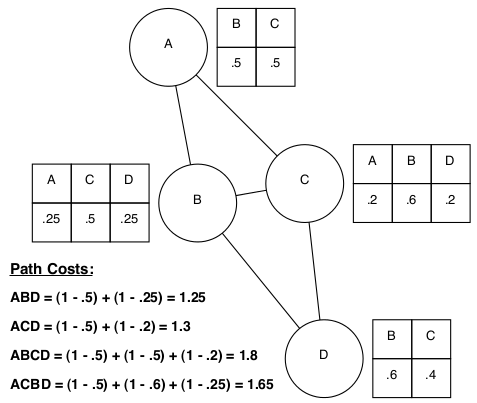
\includegraphics[width=250px]{pathcost.png}
\caption{Cálculo de costos de caminos en MaxProp \cite{mprop}}
\label{fig:pathcost}
\end{figure}

Además, los paquetes a enviar son ordenados según el número de saltos que han realizado, y una vez pasado un cierto umbral, ordenados por la probabilidad de entrega, calculada a partir del grafo. Así, los mensajes se van descartando cuando ya llevan muchos saltos, o cuando su probabilidad de entrega es muy baja, mientras se prioriza el esparcir mensajes nuevos al comienzo, independiente de su probabilidad de entrega.

Al encontrarse dos nodos, intercambian sus cálculos de pesos y los paquetes de mayor prioridad, aumentando el número de saltos de éstos. Los nodos guardan una cantidad considerabled de información de los paquetes que han pasado por él, y cada paquete a su vez guarda información de los nodos por los que ha pasado por lo que se requiere una capacidad de almacenamiento alta, lo que no resulta problemático en redes vehiculares pero potencialmente sí en otros contextos.

MaxProp logra buenos resultados en pruebas usando trazas reales de buses, concluyendo que funciona mejor que el protocolo donde se conocen los encuentros y por tanto el grafo óptimo. En \cite{mprop2} se comparó este algoritmo con Spray and Wait y PRoPHET, usando un movimiento \emph{Shortest
Path Map Based Movement}, donde MaxProp no destacó en rendimiento, y se observó que tiene un gran overhead en sus transmisiones. 

%replicacion, probabilista
\subsubsection{RAPID}
RAPID\cite{rapid} es un protocolo diseñado para priorizar en el enrutamiento cierta métrica previamente determinada, replicando los paquetes hasta que lleguen a su destinatario. Para esto, se traduce la métrica de enrutamiento en utilidades por paquete, con tal de determinar en cada oportunidad de transferencia si la utilidad marginal de replicar el paquete justifica los recursos utilizados para ello, con la estructura de un algoritmo online.

Para realizar estos cálculos, RAPID utiliza un canal de control para intercambiar información de la red entre nodos, usando sólo una fracción del ancho de banda disponible, pues se sabe que los protocolos que conocen las condiciones de la red funcionan mejor \cite{rapid19}, y que los ACK en replicación mejoran las tasas de entrega, quitando paquetes innecesarios de la red. Los nodos usan este canal para intercambiar \emph{metadata} que incluye el número y ubicación de réplicas de los paquetes, y el tamaño de transferencias anteriores. Aunque esta información es inexacta, mejora bastante su desempeño.

Al funcionar como algoritmo online, la métrica seleccionada debe expresarse como una función de utilidad, por ejemplo, para minimizar el delay promedio de la red se define la utilidad de un paquete como
$ U_i = -D(i)$,
dado que el delay esperado del paquete es su contribución a la métrica. El delay, por su parte, se estima considerando el tiempo desde su creación, el tiempo esperado para ser entregado y el número de nodos que poseen réplicas del paquete. Al utilizarse trazas vehiculares ---donde modelar los tiempos de encuentro de buses es difícil ya que cambian de ruta generando ruido--- la estimación del delay consideró una distribución exponencial, es decir, la probabilidad de que $u$ y $v$ se encuentren es
$$1-e^{-\lambda t}$$
donde $1/\lambda$ es la duración inter-contacto entre $u$ y $v$, que a su vez debe ser estimada.

En la prueba realizada usando trazas de buses RAPID resultó tener mejores resultados que Spray-and-Wait y PRoPHET con métricas de delay promedio, delay máximo y tasa de entrega. Además, se observa que RAPID tiene un mejor desempeño que MaxProp por su flexibilidad, rapidez y tasa de entrega.



 \section{Forwarding} 
 Los mensajes son entregados a otro nodo cuando es considerado un mejor candidato para llegar al destinatario que el nodo actual. Dentro de esta categoría, destacaremos dos por tomar información de encuentro o evaluaciones sociales de cómo se comportan los nodos. Cabe mencionar que existen otras estrategias, como las de Geolocalización, pero que no consideraremos por resultar inviables en un contexto minero.
 
  \subsection{Historia de Encuentros}
  Se utiliza la información de los encuentros entre nodos para determinar cuáles tienen mejores probabilidades de entregar un mensaje a un cierto nodo de destino. Esta historia puede ser local ---que un nodo sólo recuerde sus propios contactos--- o global ---que se transfiera la información de todos los nodos a cada nodo. Aunque lo segundo es más preciso para cualquier estimación, es también más difícil y más costoso.
  
%forwarding, historia de encuentros, prob. semi-markov
\subsubsection{PER}
PER\cite{per} es un protocolo probabilista de reenvío. Se basa en estrategias para predecir el futuro de la red, como probabilidad de entrega de mensajes o estimación del próximo encuentro con un nodo. PER determina el próximo salto de los mensajes considerando la distribución de probabilidad de los próximos contactos para maximizar la probabilidad de entrega al destinatario final. Se utiliza un proceso \emph{semi-markov} para predecir la distribución de probabilidades del tiempo de contacto y de la probabilidad de encuentro de dos nodos, por lo que es complejo de implementar.
Su uso en simulaciones determina que tiene una mejor tasa de entrega que los protocolos usuales de enrutamiento, con una latencia normal pero con energía y ancho de banda grandes. No requiere mucho almacenamiento al realizar \emph{forwarding}, pero sí capacidad de procesamiento de los nodos.

%forwarding, patron de movimiento
\subsubsection{SMART}
SMART\cite{smart} es también una evolución de Spray-and-Wait, que incorpora el concepto de \emph{compañeros de viaje} de nodos --- es decir, nodos que frecuentemente se encuentran --- para mejorar la probabilidad de entrega sin propagar ni la historia de encuentros ni las probabilidades de entrega. Cada nodo propaga frecuentemente pequeños mensajes para declarar su presencia, con lo que cada nodos logra conocer con cuáles nodos comparte más frecuentemente. Con esta información un nodo envía $f_1-1$ copias del mensaje utilizando \emph{binary spray}, preguntando a los nodos que encuentra si son compañeros del destinatario. Al encontrar un compañero, éste a su vez envia $f_2-1$ mensajes a los compañeros del destinatario, esperando encontrarlo con mayor probabilidad que aquellos que no reconocen al destinatario como compañero. Los valores $f_1$ y $f_2$ son fijados en el protocolo, y deben adecuarse según el movimiento y topología donde se utilice.

\begin{figure}[h]
\centering
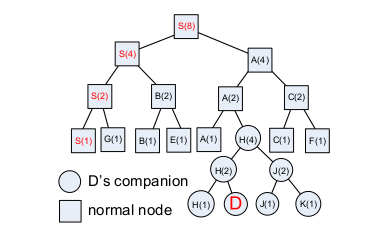
\includegraphics[width=200px]{smart.png}
\caption{Enrutamiento de SMART con $f_1 = 8$ y $f_2 = 4$ \cite{smart}}
\label{fig:smart}
\end{figure}

Esta estrategia es interesante al no requerir enviar información de encuentros de los otros nodos logrando incorporarla localmente. En simulaciones se observa que tiene una alta tasa de entrega (90\%), comparable a Epidemic, muy poco \emph{overhead} comparado a Epidemic, y una latencia menor que \cite{sandw}, aunque mayor que Epidemic, resultando ser una buena estrategia de incorporar inteligencia sin mucho procesamiento, a diferencia de Spray and Focus.
 
  \subsection{Información social}
  Se toma como hipótesis que los nodos de la red presentan ciertos patrones de comportamiento que influyen en su movilidad y sus contactos, por lo que se utiliza esta información para definir los roles de los nodos en la red desde una perspectiva social. Este tipo de estrategias requiere un conocimiento mayor de la topología donde se aplicará, puesto que su enrutamiento depende fuertemente de una correcta inferencia del contexto.

%orbitas sociologicas, hubs, prediccion global movilidad, forwarding
\subsubsection{SOLAR}
SOLAR \cite{solar} es un protocolo que considera una predicción de la movilidad de los nodos de manera global, dada la dificultad de mantener información detallada de movimientos individuales en DTNs. Considera un patrón de movimiento \emph{orbital} en torno a varios \emph{ejes}, denominado \emph{parcialmente determinista}, a diferencia de movimientos deterministas como satélites o buses considerados en otros protocolos.

El patrón de movimiento orbital considera \emph{hubs} o ejes asociados a un tiempo de estadía, definiendo un conjunto de éstos la Órbita Inter-Ejes (IHO en inglés), considerando así el movimiento dentro de los hubs como entre éstos, los cuales a su vez pueden ser otros patrones de movimiento, como se muestra en la Figura \ref{fig:orbit}

\begin{figure}[h]
\centering
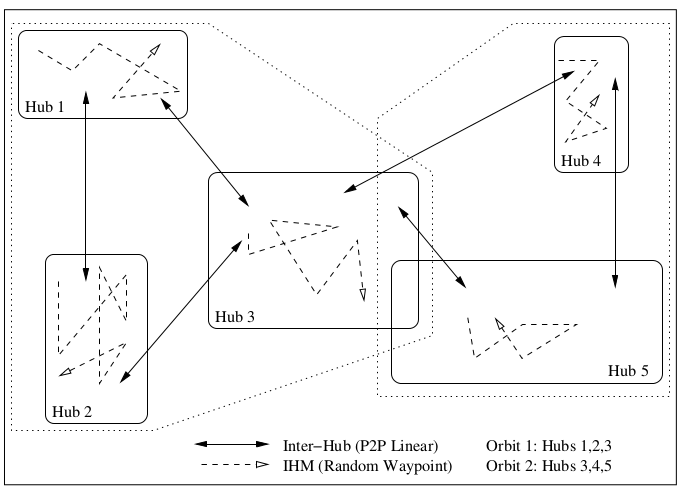
\includegraphics[width=200px]{solar-orbit.png}
\caption{Modelo ORBIT aleatorio \cite{solar}}
\label{fig:orbit}
\end{figure}

Cuando los nodos se encuentran, intercambian sus IHOs en su saludo, volviéndose \emph{conocidos} entre sí. Así, para enrutar, el nodo busca si conoce su IHO. Si lo hace, envía paquetes a sus ejes. Si no, pregunta a sus conocidos si lo conocen, hasta encontrar su IHO. Si además se conoce la posición aproximada de los ejes, se puede utilizar un protocolo geográfico para llegar al destino, que obtiene mejores resultados que otros protocolos.
Decidir el mejor conjunto de nodos \emph{conocidos} es un problema que puede reducirse a \texttt{Set Cover}, que es NP-Hard, volviendo costoso buscar un buen conjunto y debiendo utilizar aproximaciones.
En la implementación simplificada de este protocolo se obtiene desempeño comparable a Epidemic y con menos \emph{overhead}, pero al ser bastante básica deja mucho espacio para mejoras.

%forwarding, social, hierarchical
\subsubsection{BUBBLE}
BUBBLE \cite{bubble} es un protocolo social, donde en vez de considerar los patrones de movilidad de los nodos busca evaluar sus relaciones e importancia en la red, la cual es menos cambiante que su patrón de movimiento. Para realizar esto, BUBBLE toma dos parámetros: las \emph{comunidades} formadas por la cooperación entre nodos, y la \emph{centralidad} de un nodo dentro de su comunidad, es decir, qué tan popular es, determinado por el número de interacciones de éste, que también logra capturar el rol que puede tener un nodo en la red.

El protocolo requiere tres valores de cada nodo: su comunidad $c$, su ranking local $l$ en su comunidad, y su ranking global $g$ entre todos los nodos del sistema. Al enviar un mensaje $m$, el protocolo evalúa si ya encontró la comunidad de destino. Si es así, intenta avanzar por los nodos de mayor $l$. En caso contrario, intenta avanzar por los nodos de mayor $g$, hasta que el mensaje llegue al destino o alcance su timeout. 

Una dificultad de este algoritmo está en evaluar la existencia de comunidades y centralidad en éstas. Para ello se utilizan dos algoritmos de detección de comunidades: \texttt{K-CLIQUE} de Palla et al. y \emph{Weighted Network Analysis} (WNA) de Newman \cite{bubble24}. \texttt{K-CLIQUE} puede reconocer comunidades superpuestas, pero al ser para grafos binarios no puede asignar pesos a los enlaces. Por su parte, WNA puede asignar pesos pero no encontrar superposiciones, por lo que se combinan ambos. Este análisis, además, debe hacerse de manera distribuida, donde cada nodo debe encontrar su comunidad y calcular su centralidad, para lo que se introduce DiBuBB, algoritmo distribuido que aproxima estos valores, encontrando correlación en el número de nodos únicos visto en una unidad de tiempo con la centralidad, siendo por tanto un buen estimado.

BUBBLE logra buenos resultados en simulaciones utilizando varias trazas de movimientos humanos reales, obteniendo resultados similares a PRoPHET en tasa de entrega, pero con menor \emph{overhead}. BUBBLE promete obtener buenos resultados tanto en comunidades de estructura plana, como las de prueba, como en estructura jerárquica, que se adapta directamente a la centralidad social.


\newpage
\part*{Patrones de movilidad en DTNs}

En la simulación de DTNs, los patrones de movilidad son fundamentales para emular el comportamiento de personas y paquetes de manera verosimil, lo que es importante para poder determinar cómo se comportará un protocolo en su contexto real de implementación.

La transmisión ocurre cuando los nodos se encuentran entre sí, intercambiando información de control y mensajes si los protocolos lo consideran apropiado. El tiempo que tarda un nodo en entrar en contacto con otro se denomina \emph{tiempo de encuentro}. El tiempo de contacto entre ellos, lo cual definirá las posibilidades de enviar datos entre sí mientras dure el contacto, se denomina \emph{tiempo de contacto}. Si no pueden concluir el intercambio de paquetes en ese tiempo, deben esperar hasta entrar nuevamente en contacto. Esto se denomina \emph{tiempo inter-encuentros}. Para realizar un análisis realista es necesario conocer estadísticamente estas tres cantidades. 

Los modelos de movilidad son generados utilizando trazas reales y modelos sintéticos con respaldo teórico, con lo que se busca lograr escenarios realistas. Generalmente, los distintos protocolos son evaluados utilizando ciertos modelos tradicionales, y se utilizan características especiales para afinar y demostrar mejoras en usos específicos de los protocolos, como redes vehiculares o de personas en contextos específicos. Se presentan algunos de los modelos más utilizados, clasificados en tres categorías.

La más simple y tradicional familia de modelos de movimiento son los de \emph{Random Mobility} o movimiento aleatorio, de los cuales destacan:

\begin{enumerate}
	\item Random Walk (RW)
	\item Random Walkway Point (RWP) 
	\item Random Direction (RD)
	\item Levy Walks (LW) 
\end{enumerate}

Otro tipo de modelos es derivado de patrones aleatorios, pero limitados a un mapa. En estos modelos los datos del mapa son incluídos utilizando el formato \emph{Well Known Text} (WKT), utilizando ampliamente en modelos de información geográfica (GIS). Algunos de los más populares modelos basados en mapas son:

\begin{enumerate}
	\item Map-Based Mobility Model (MBM)
	\item Shortest Path-Based Map (SPBM)
	\item Route-Based Map (RBM)
	\item Manhattan Mobility Model (MMM)
\end{enumerate}

En aquellas aplicaciones de DTNs donde los nodos son humanos, animales o vehículos que poseen ciertos patrones de movimiento, es posible explotar estos patrones para mejorar el desempeño de los protocolos. Estos patrones incluyen recorridos y modelos sociales basados en el comportamiento humano, por ejemplo:

\begin{enumerate}
	\item Community-Based Mobility Model (CMM)
	\item Time-Variant Community Model (TVCM)
	\item Working Day Movement (WDM)
	\item General Social Mobility Model (GeSoMo)
	\item Disaster Scenario (DS)
\end{enumerate}

Estos patrones de movilidad pueden ser configurados por cada nodo, por lo que es posible combinar varios modelos de movimiento en una simulación. A continuación se describe cada modelo en profundidad, analizando sus características y los escenarios que buscan representar.


\section{Modelos de Movilidad Aleatorios}

\subsection{Random Walk}
En el modelo Random Walk, cada nodo se mueve de manera impredecible, escogiendo un destino aleatorio y avanzando hacia él con dirección y velocidad de un rango predefinido. Una nueva dirección es asignada cada vez que el nodo llega a su destino. Cada nodo de la red se comporta de manera independiente a los otros. Este modelo no mantiene memoria de la movilidad anterior, ya que no lleva registro de los patrones formados por la ubicación y movimiento de los nodos, siendo su movimiento independiente de su historia. Esto puede generar algunos movimientos poco realistas como paradas abruptas o vueltas cerradas. A pesar de ello, este modelo ha sido popular al evaluar protocolos DTN por su estabilidad en la distribución de los parámetros de movilidad por comportarse de manera estable.

\subsection{Random Walkway Point}
Este es otro modelo básico y simple utilizado frecuentemente en simulaciones. RWP incluye una pausa después de concluir un segmento de caminata aleatorio. La dirección, velocidad y tiempos de pausa son tomados de una distribución uniforme. Un nodo se mueve a un destino a velocidad constante, se queda ahí por un momento, y luego toma un nuevo destino aleatoriamente. Este modelo es fácil de analizar y de implementar, por lo que es también ampliamente utilizado para evaluar protocolos a pesar de su movimiento artificial. Se presenta a veces un problema de distribución no uniforme en los nodos, lo cual complica su análisis y su uso.

\subsection{Random Direction}
Este modelo de distribución aleatoria de direción soluciona el problema encontrado en RWP. En este modelo, un nodo obtiene un ángulo aleatorio y se mueve en esa dirección hasta encontrar la frontera del área de simulación. Al encontrarla, el nodo se detiene por un tiempo específico y luego escoge una nueva dirección, moviéndose nuevamente. Este modelo es más consistente que otros modelos aleatorios, y ofrece distribuye uniformemente los nodos en el área de simulación. Existen muchas variantes de RD, donde se incorporan factores para manejar la duración de la caminata y diferentes efecto al llegar a la frontera.

\subsection{Levy Walks}
Este modelo es similar a RW, pero donde las variables de movilidad son tomadas de una distribución de ley potencial. Este modelo es capaz de generar distribuciones de tiempo inter-contacto similar a trazas reales, pero sin capturar las relaciones entre nodos. Otra característica es la alta \emph{difusividad}, es decir, el desplazamiento en el tiempo tiene una alta varianza (16). Una variante de este modelo es Truncated Levy Walks, que utiliza distribuciones truncadas de Paretto para emular la movilidad en una área confinada y distribuciones truncadas de Paretto para áreas externas. TLW entrega representaciones más realistas de los patrones estadísticos encontrados en la movilidad humana mientras preserva la simplicidad de los modelos aleatorios.


\section{Modelos Limitados por Mapas}

\subsection{Map-Based Mobility Models}
Este modelo aleatorio basado en mapas es un derivado de Random Walk. Aquí, un nodo se mueve en una dirección siguiendo los caminos determinados por el mapa dado. Esto permite distinguir entre distintos nodos, como automóviles y peatones, separando los caminos posibles para cada categoría. Los nodos avanzan por un segmento hasta encontrar el fin de una calle o una intersección, donde deciden aleatoriamente una nueva dirección, pero no vuelven por donde venían. Al viajar una cierta distancia, los nodos se detienen por un tiempo y luego continúan su viaje. Al concluir la simiulación, se obtiene una distribución aleatoria de los nodos en todo el mapa. Una limitación de este modelo es que los nodos siguen caminos definidos por el mapa aleatoriamente, generando patrones de movimiento poco similares a las trazas reales. 

\subsection{Shortest Path-Based Map Mobility Model}

Este modelo es una mejora de MBMM, donde los nodos viajan a un cierto destino en el mapa siguiendo el algoritmo de Dijkstra de caminos mínimos para encontrar la mejor ruta a su destino. Todas las ubicaciones del mapa tienen la misma probabilidad de ser escogida, pero también se incluen Puntos de Interes (\emph{POIs} en inglés), cuya probabilidad es configurable. Estos POIs son también agrupables. Esto otorga una gran ventaja al modelar lugares donde la gente tiene a reunirse, como restaurantes, supermercados o atracciones turísticas. Aún así, no asegura tiempos inter-contacto ni distribuciones de tiempo de contacto similares a las trazas reales cuando el número de nodos es pequeño.

\subsection{Route-Based Map Mobility Model}

Este modelo añade la asignación de rutas predefinidas en el mapa a algunos nodos. Esto genera un mejor desempeño al simular, por ejemplo, el transporte público, donde las rutas son conocidas de antemano. En este modelo, las rutas en el mapa contienen muchos puntos denominados paradas en la ruta, donde los nodos esperan cierto tiempo hasta avanzar a la próxima parada. Para llegar a su destino, los nodos siguen el camino mínimo. Existen algunas variantes, como Street Random Waypoint (STRAW) donde los nodos viajan acorde a un tráfico vehicular realista en caminos definidos por un mapa real.

\subsection{Manhattan Mobility Model}

MMM es un modelo basado en mapa ampliamente utilizado para imitar el movimiento de áreas urbanas. El mapa de MMM genera una grilla de lineas horizontales y verticales, que representa las calles en el mapa. Los nodos tienen permitido moverse por estas lineas, y cambiar su dirección con cierta probabilidad al llegar a una intersección, dando al nodo cierta libertad. La configuración de probabilidades al llegar a intersecciones influye en la dependencia espacial y temporal de los nodos, por lo que su análisis matemático puede complicarse.


\section{Modelos de Movilidad Social}

\subsection{Community-Based Mobility Model}

El modelo basado en comunidad es el primero en tomar en cuenta una red social. En CMM, los nodos se agrupan como amigos pertenecientes a la misma comunidad, y no-amigos que están en otras comunidades. Al principio, el área de movimiento se divide en regiones como una grilla, y cada comunidad es asignada a una celda de la grilla. Los nodos se mueven entre comuniades basado en un factor de atracción de nodos, lo que puede generar una segregación en el comportamiento de éstos. Algunas variantes incluyen relaciones entre comunidades distintas de la propia, donde la probabilidad de que un nodo se mueva de su comunidad a otra es proporcional a la amistad con los nodos de aquella comunidad.

\subsection{Time-Variant Community Model}

En este modelo, el plano de simulación se divide en territorios asignados a cada comunidad. Cada nodo es asignado una velocidad global, y viaja entre comunidades usando probabilidades de transición siguiendo una Cadena de Markov. Esta configuración de comunidades y probabilidades de transición se mantienen fijas por un cierto período de tiempo, que luego cambian. Cada nodo puede poseer distintas configuraciones, capturando los sesgos que puedan existir en las preferencias de éstos. Esta estrategia logra dar más realismo al modelo, y logra aproximarse a trazas reales con una selección apropiada de parámetros.

\subsection{Working Day Mobility Model}
 
Este modelo refleja un patrón de movilidad más real al considerar tres actividades realizadas por los humanos: dormir en casa, trabajar en una oficina y salir con amigos en las tardes. Distintos sub-modelos se pueden utilizar en cada una de estas actividades. Los nodos hacen transiciones entre los tres modelos según el tipo de nodo y la hora del día. Además, el modelo cuenta con diferentes modelos de transporte, ya que pueden caminar, conducir o viajar en bus entre los distintos sub-modelos, y pueden moverse aislados o en grupo. Al ocurrir a diferentes velocidades se aumenta la heterogeneidad de los nodos. El concepto social de WDM no es capturado en modelos simples como RWP, y se observa que el tiempo inter-contacto y la distribución de tiempo de contacto son similares a trazas del mundo real.

\subsection{General Social Mobility Model}

GeSoMo es un modelo de movilidad social que separa un modelo central de una explicación estructural de la red social en la simulación. Este diseño permite a GeSoMo generalizar ampliamente, aceptando redes sociales como input. Basado en esto, GeSoMo genera una traza organizada por el movimiento de cada nodo individual. Esta traza genera encuentros entre nodos acorde a su relación social considerado atracción y repulsión de nodos, y atracción de ubicaciones. Esta estructura permite cambiar la interacción social sin cambiar GeSoMo. Sus resultados de movilidad son coherentes con datos empíricos que describen comportamiento y movimiento social del mundo real.

\subsection{Disaster Scenario}

El escenario de desastres pretende simular la movilidad experimentada en el rescate posterior a una emergencia. Considera un conjunto de sub áreas independientes y disjuntas que representan .............. Así, el escenario consiste en un área de simulación, un conjunto de sub-áreas, y un conjunto de obstáculos que limitan la movilidad. 


\newpage
\part*{Modelo de movilidad en minas subterráneas}

\documentclass[10pt,preprint,onecolumn]{article}
\usepackage[utf8]{inputenc}
\usepackage[spanish]{babel}
\usepackage[T1]{fontenc}
\usepackage{mathtools, comment, url, hyperref}
\usepackage[cm]{fullpage}
\usepackage{setspace}
\usepackage{float}
\usepackage{wrapfig}
\usepackage[pdftex]{graphicx}
\usepackage{listings}
\usepackage{amsmath}
\usepackage{tikz}
\usetikzlibrary{automata,arrows,positioning,calc}
\usepackage{caption}
\usepackage{cite}
\usepackage{subcaption}
\usepackage{lscape}
%\restylefloat{figure}
\singlespacing

\begin{document}

\begin{comment}

A continuación se presenta una descripción en mayor detalle del modelo escogido como referente, Disaster Scenario, tomando en consideración la manera de utilizarlo para el escenario de minería subterránea.

\section{Disaster Scenario}

\begin{figure}[H]
    \centering
    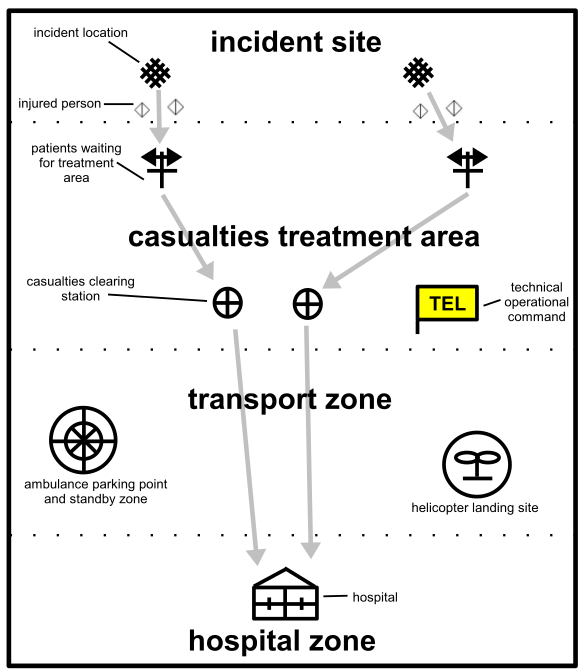
\includegraphics[width=280px]{disaster.png}
    \caption{Representación del escenario de desastre}
    \label{fig:disaster}
\end{figure}


Se define formalmente un escenario de desastre $S$ como un área de simulación dividida en áreas tácticas disjuntas: la zona del incidente (IL), zona de pacientes esperando tratamiento (PWT), estación de rescate de víctimas (CCS), punto de estacionamiento de ambulancias (APP), y un centro técnico operacional (TOC). La simulación coonsiste en un área $F$, un conjunto de áreas tácticas $R$, y un conjunto de obstáculos $H$. Un área táctica $r \in R$ es una tupla definida como

$$ r = (l_r, P_r, e_r, a_r, N_r^{stat}, V_r^{stat}, T_r^{stat}, G_r^{stat}, N_r^{trans}, V_r^{trans}, T_r^{trans}, G_r^{trans}, Z_r^{trans})$$

donde
\begin{enumerate}
\item $l_r \in \{IL, PWT, CCS, APP, TOC\}$ es la clasificación del área táctica,
\item $P_r \subset F$ es una parte poligonal del área F,
\item $e_r$ y $a_r$ son dos puntos al borde de $P_r$, de entrada y salida respectivamente,
\item $N_r^{trans}$ y $N_r^{stat}$ son dos conjuntos de nodos
\item $V_r^{trans}$ y $V_r^{stat}$ son los intervalos de velocidad $[v_{min}, v_{max}]$de los nodos en $N_r^{trans}$ y $N_r^{stat}$,
\item $N_r^{trans}$ y $N_r^{stat}$ son los intervalos de tiempo $[t_{min}, t_{max}]$ para las pausas de los nodos en $N_r^{trans}$ y $N_r^{stat}$,
\item $N_r^{trans}$ y $N_r^{stat}$ son los tamaños de los grupos de nodos en $N_r^{trans}$ y $N_r^{stat}$,,
\item $Z_r$ es la secuencia de puntos o ciclo de movimiento de los nodos de transporte.

\end{enumerate}

Cada área táctica $r$ tiene un punto de entrada $e_r$ y un punto de salida $a_r$. Los nodos que transportan pacientes pueden dejar las áreas sólo mediante estos puntos. Este modelo es motivado por los puntos de registro de entrada y salida para los pacientes. Cada nodo es asignado a un área táctica, pudiendo ser \emph{estacionario}, es decir, permanece dentro de su área táctica y sólo se mueve dentro de $P_r$; o es un nodo de transporte, acarreando pacientes entre distintas áreas basado en el movimiento dado por $Z_r$. Los nodos estacionarios se denominan $N_r^{stat}$, mientras que los de transporte se denominan $N_r^{trans}$. 


\subsection{Definición de las zonas}

Para los centros técnicos operacionales y estaciones de rescate, se asume que los nodos son todos estacionarios, es decir,

$$\forall r \in R| l_r \in \{CSS, TOC\} : N_r^{trans} = \emptyset, Z_r^{trans} = \emptyset$$

Por otra parte, las zonas de incidentes consiste exclusivamente de nodos de transporte, es decir,

$$\forall r \in R| l_r \in \{IL\}: N_r^{stat} = \emptyset$$

Los nodos de transporte $n \in N_r^{trans}$ de la locación de incidentes comienzan en el punto $a_r$. Allí selecciona un punto aleatorio $rand \in P_r$ y se mueve a ese punto. Desde allí se mueve hasta el punto de salida $a_r$ y se mueve hacia un punto aleatorio de la zona \emph{pacientes esperando tratamiento}, $e_{PWT_{rand}}$. Finalmente, se mueve de vuelta al punto $a_r$. Este ciclo modela el recoger a un paciente de la zona de incidentes y llevarlo a la zona de tratamientos. En los puntos $rand$ y $e_{PWT_{rand}}$ se realiza una pausa de acuerdo a una distribución uniforme tomada de $T_r^{trans}$. Con esto se modela la primera asistencia a los pacientes 


\textbf{Pacientes esperando tratamiento:} $r \in R | l_r = PWT$
Se realiza un ciclo entre $PWT$ y $CCS$ o estación de rescate de víctimas. 

\textbf{Estacionamiento de ambulancias:} $r \in R | l_r = APP$
Los nodos de transporte se mueven tras entrar al escenario por la entrada $e_r$, a un punto aleatorio $rand \in P_r$ dentro del área. Después de una pausa de un tiempo aleatorio, se abandona el estacionamiento usando el punto $a_r$. Desde ahí, se mueven a la salida $a_r$, desde donde se mueven a una salida $a_{CSS_{rand}}$ de una estación de rescate de víctimas (CSS) aleatoria. Realizan otra pausa en este lugar, y luego abandonan el escenario.
Este movimiento describe ambulancias que entran, se estacionan, recogen a pacientes para llevarlos al hospital y abandonan el escenario. 

\subsection{Manejo de obstáculos}

Se considera la zona de simulación $F$ como planar y estática, con un conjunto de obstáculos poligonales simples (sin hoyos ni autointersecciones) $H$. Se utilizan métodos de planificación de movimiento de robots para decidir las rutas. Se asume que las áreas tácticas $P_r$ son también polígonos simples.

Para encontrar el mejor camino, se utilizan grafos de visibilidad. Esto es, un grafo donde sus vértices son los vértices de los obstáculos, y existe un arco entre dos vértices si se puede "ver", es decir, no intersecta el interior de ningún obstáculo. Se añaden las entradas y salidas de las zonas como vértices al grafo. Luego de calcular el grafo, se asignan pesos según la distancia euclidiana. Con esto, se puede utilizar el algoritmo de Dijkstra para encontrar el conjunto de arcos que componen el mejor camino.

\newpage
\end{comment}

\section{Escenario de Mina Subterránea}

\subsection{Escenario}

\subsubsection{Descripción}

El escenario está compuesto por las siguientes zonas poligonales y adyacentes, cuya distribución se puede ver en la Figura \ref{fig:underground}. Por simplicidad, el dibujo se representa con rectángulos. Las áreas se conectan entre ellas con puntos de acceso específicos.

\begin{enumerate}
    \item \textbf{Centro Civico (CEC):} Es el área donde comienza la comunicación hacia el exterior, y el punto inicial y final de los operarios de la mina. Esta zona cuenta con conectividad total hacia el exterior, por lo que se puede considerar la zona final para la información.
    
    \item \textbf{Zona de Acceso (ACC):} El área de ingreso que conecta las zonas laterales y de extracción. Esta zona cuenta con conectividad hacia el centro cívico, pero con baja densidad de antenas.
    
    \item \textbf{Zona de extracción (EXT):} Es el área más relevante de la mina. No cuenta con conectividad. En esta zona se concentra el movimiento de los distintos nodos.
    Está conformado por una estructura de grilla que representan los posibles caminos dentro del área. Los ejes verticales están completamente despejados, mientras los ejes horizontales contienen obstáculos en el $70\%$ de los casos\footnote{Esto es una estimación muy arbitraria, ya que no pude conseguir un número }. En los bordes superior e inferior se ubican entre 1 y 4 DUMP, puntos de descarga, dependiendo del tamaño de la mina.
        
    \item \textbf{Zonas laterales(LAT):} Representan los accesos a los niveles superiores e inferiores de la mina donde ocurren otras operaciones, tal como la explotación en el nivel superior o el chancado primario en el nivel inferior. Por simplicidad topológica, las consideraremos áreas a los costados de la zona de Acceso.

    \item \textbf{Zona de mantención (MAN):} Representan los lugares donde se realiza mantención y actividades operativas, como carga de combustible. Estas zonas son aledañas a la zona de extracción EXT, y puede serlo a la zona de acceso ACC. En el escenario pueden existir 1 o 2 zonas de mantención, dependiendo del tamaño de la mina.
    
\end{enumerate}

\begin{figure}[H]
    \centering
    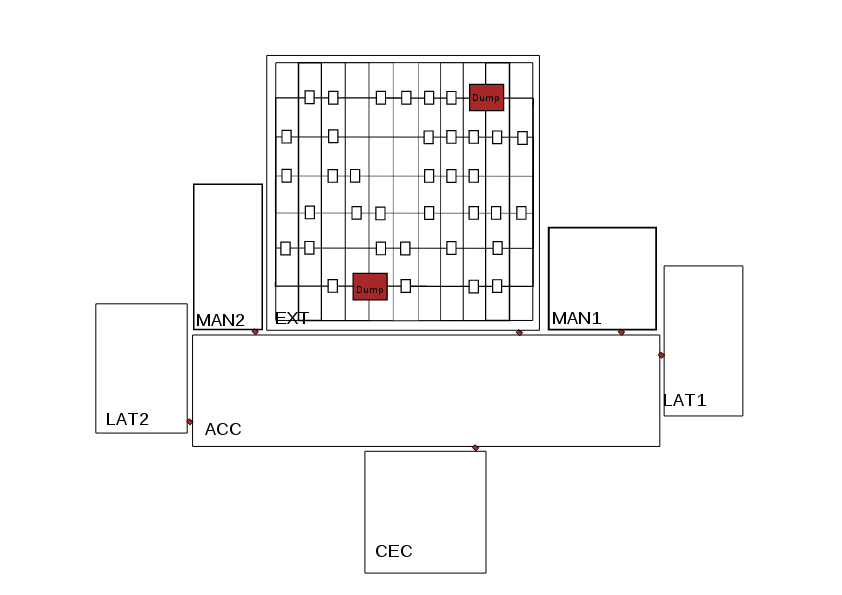
\includegraphics[width=400px]{underground2.png}
    \caption{Areas y conexiones del modelo de mina subterránea.}
    \label{fig:underground}
\end{figure}

\subsubsection{Restricciones}

Existen algunas restricciones que se imponen en el diseño de las distintas áreas que se listan a continuación.

\begin{itemize}

    \item El tamaño de la mina es una variable de la que dependerán las dimensiones de las distintas áreas, y en particular la zona de extracción, el número de DUMP y el número de áreas MAN. Además, el tamaño de la mina define el número de nodos dentro de ella. Se considerará un número entre 1 y 5, siendo 1 una mina pequeña y 5 una mina muy grande.
    
    \item La zona de extracción tiene exclusividad temporal para las LHDs, es decir, una vez trazada una ruta de la LHD, otras LHDs u operarios no pueden utizar esa ruta. 
    
    \item Existen interrupciones por explosión, que cierran y paralizan temporalmente la operación en un punto de intersección, sus 2 caminos aledaños verticales, y sus 2 aledaños horizontales. Estas pausas son breves y permiten continuar la operación normalmente. Su frecuencia tiene una distribución normal en torno a 1 cada 3 horas. 
    
\end{itemize}

\subsection{Movilidad}

\subsubsection{Tipos de Nodos}

\begin{enumerate}
    %personas
    
    \item Operarios (OP): Son los encargados del funcionamiento global. Son del tipo estático, trabajando en sólo una zona: MAN o CEC. Se mueven en grupos entre 1 y 3 personas, sólo dentro de
    
    \item Operarios de Mantenimiento (OM): Son los encargados de realizar actividades breves de mantenimiento en distintas zonas. Se mueven en grupos de entre 3 y 5 entre todas las áreas, realizando trabajos (pausas) en todas las zonas: CEC, ACC, EXT, LAT y MAN.
    
    \item Supervisores (SU): Son quienes supervisan las actividades. Son entre 1 y 2, y recorren las distintas áreas de manera pseudoaleatoria siguiendo decisiones representadas como una cadena de Markov\footnote{El motivo de usar una cadena de Markov para supervisores, es que un ciclo sería demasiado determinista, pero aleatorio sería irreal; una cadena de markov permite un buen orden con alta probabilidad, pero permite incorporar casos distintos que son frecuentes. Esto es totalmente arbitrario de lo que me han comentado 2 supervisores de cómo es, definitivamente necesita validación.}, como se ve en la Figura \ref{fig:markov}
    
    %maquinas
    
    \item Camionetas (CA): Son equivalentes a los operarios de mantención, pero a una velocidad mayor y se desplazan individualmente. 
    
    \item Load, Haul, Dump Machines (LHD): Son las máquinas de carga, recorrido y descarga. Su movimiento se restringe a las zonas EXT y MAN. Su movimiento sigue el siguiente algoritmo\footnote{Mi propuesta es que se use una distribución de Poisson para la pausa de las máquinas, ya que es canónica para modelar en torno a un promedio los sucesos raros: en nuestro caso, que una mantención resulte ser una falla que requiere más tiempo de pausa.}:
    \end{enumerate}
    \begin{verbatim}
definir DUMP de la LHD
for(random 50-200):
    seleccionar punto aleatorio P en el área EXT no reservada.
    for(random 10-30):
        ir a P. pausa aleatoria ~15s
        recorrer mejor ruta sin obstáculos para llegar a DUMP. v=12km/h
        ir a DUMP. pausa aleatoria ~5s
    end
    ir a la zona de mantención más cercana, a través de la zona de $ACC$. 
    Pausa en torno a 30m según distribución de Poisson
end
\end{verbatim}

\begin{enumerate}
  \setcounter{enumi}{5}
    \item Martillos picadores (MP): Son estáticos y se ubican en sobre los puntos de DUMP. Dada su operación remota, se considera que son puntos de acceso a la red \emph{backbone} cableada.
\end{enumerate}


\begin{figure}
\begin{center}
\begin{tikzpicture}[->, >=stealth', auto, semithick, node distance=9cm]
\tikzstyle{every state}=[fill=white,draw=black,thick,text=black,scale=0.8]
    \node[state]    (A)                     {CEC};
    \node[state]    (B)[right of=A]   {ACC};
    \node[state]    (C)[below right of=A]   {EXT};
    \node[state]    (D)[above of=B]   {LAT$_i$};
    \node[state]    (E)[below right of= B]  {MAN$_m$};
\path

%centro civico
(A) edge[loop left]             node{$0.6$}                                 (A) %me quedo en CC
    edge[bend left]             node{$0.4$}                                 (B) %ir al área de decision
    
%acceso    
(B)
    edge[bend left]             node{$0.3$}                                 (A) %volver al CC
    edge[bend right, left]      node{$0.3$}                                 (C) %ir al area de extraccion
    edge[bend left, left]       node{$\frac{0.2}{|M|}, \forall m \in M$}    (D) %ir a laterales
    edge[bend left, right]      node{$\frac{0.2}{|I|}, \forall i\in I$}     (E) %ir a una de las mantenciones
    
%extraccion
(C) edge[loop right]            node{$0.2$}                                 (C) %ir a otro punto en el área de extracción
    edge[bend right, right]     node{$0.2$}                                 (B) %volver al al acceso
    edge[bend left, above]      node{$0.2$}                                 (A) %volver al CC
    
%laterales
(D) edge[bend left, right]      node{$0.3$}                                 (B) %volver al acceso
    edge[bend right, above] node{$0.7$}                                 (A) %volver al CC
    
%mantencion
(E) edge[loop right]            node{$\frac{0.4}{|I|}, j\neq i, j\in I$}    (E) %ir a otra mantención
    edge[bend left]            node{$0.3$}                                  (B) %volver a la zona de extracción
    edge[bend left=70]             node{$0.3$}                                 (A);%volver al CC

\end{tikzpicture}
\caption{Autómata representando transiciones para los supervisores}
\label{fig:markov}
\end{center}
\end{figure}

\newpage
\section{Definición Formal}

Formalmente, definiremos un escenario de minería subterránea como un área de simulación dividida en áreas disjuntas, de los tipos $CEC, ACC, EXT, LAT$ y $MAN$, representando las zonas previamente definidas. Las áreas $CEC, ACC$ y $EXT$ son únicas, $LAT$ son dos, y $MAN$ pueden ser 1 o 2 dependiendo del tamaño de la mina.

A diferencia del escenario de desastre, los nodos no pertenecen a un área táctica única, sino que su tipo determina su patrón de movilidad, donde todos comienzan desde el área $CEC$, exceptuando las $LHD$.
La simulación coonsiste en un área $F$, un conjunto de áreas tácticas $R$, y un conjunto de obstáculos $H$. Un área táctica $r \in R$ es una tupla definida como

$$ r = (l_r, P_r, A_r, D_r, C_r, R(t))$$

donde
\begin{enumerate}
\item $l_r \in \{CEC, ACC, EXT, LAT, MAN\}$ es la clasificación del área táctica,
\item $P_r \subset F$ es una parte poligonal del área F,
\item $A_r$ es el conjunto de puntos $a_r$ de acceso, situados al borde de $P_r$.
\item $C_r$ es el conjunto de obstáculos.
\item $D_r$ es un conjunto de obstáculos que determinan una zona de atracción para los distintos nodos.
\item $R_r(t)$ es un conjunto de obstáculos dependientes del tiempo generados por las restricciones de acceso en las distintas zonas por los nodos.
\end{enumerate}
Por su parte, los nodos y sus patrones de movilidad están definidos como:

$$ n = (t_n, d_n, V_n^{ml}, V_n^{Ml}, Z_r) $$

donde
\begin{enumerate}
\item $t_n \in \{OP, OM, SU, CA, LHD. MP\}$ es la clasificación del tipo de nodo
\item $V_n^{ml_r}$ y $V_n^{Ml_r}$ son los intervalos de velocidad $[v_{min}, v_{max}]$ para el nodo en un área del tipo $l_r$.
\item $N_n$ es el tamaño de los grupos de nodos.
\item $Z_n^{l_r}$ es el ciclo de movimiento del nodo dentro de un área de tipo $l_r$.

\end{enumerate}

\end{document}

\end{comment}
\input{movilidad/mining}
\newpage
\part*{Conectividad en entornos mineros}

%%Para determinar la comunicación existente y posible en minería, es necesario separar la minería de rajo abierto, que suele contar con redes celulares negociadas directamente con los proveedores de internet  ---exceptuando aquellas de pequeña escala y artesanal---, y la minería subterránea, donde no existen los medios de comunicación disponibles en la superficie. Por esto, ha surgido tecnología dedicada a la minería subterránea, que a su vez cuenta con una gran variabilidad de ambientes como túneles y galerías. A continuación se presenta una revisión de las características más importantes en estos ambientes, tomadas del estudio realizado por Mauricio Contreras \cite{tesis} de comunicación en minas chilenas subterráneas, y del informe interno de Codelco para Intraestructura en Minas Subterráneas\cite{doccodelco}.

\section{Características Importantes}

La comunicación en minería es fundamental para la coordinación de actividades, imprescindible para evitar accidentes que pueden ser fatales. Se hace énfasis a la comunicación de seguridad, tanto de datos tomados por sensores como de alertas para notificar un potencial problema humano que podría desencadenar una falla de mayor escala.

\begin{enumerate}
\item \textbf{Robustez:} Dado que las minas subterráneas están sujetas a potenciales colapsos y otros riesgos, la habilidad de un equipo de comunicación de emergencia de mantenerse operacional ante un accidente es fundamental. Por ello, se requiere una infraestructura de red que no se desconecte con un daño estructural.

\item \textbf{Flexibilidad:} El ambiente de las minas está continuamente cambiando por el proceso de extracción. Esto resulta en una necesidad continua de expandir y modificar la conectividad necesaria. Los sistemas que requieren un gran esfuerzo de instalación ofrecen una menor flexibilidad, pero a la vez, un sistema totalmente inalámbrico puede congestionarse al expandirse el sistema.

\item \textbf{Rango/Cobertura:} Dadas las distancias potencialmente largas entre los operarios, y el hecho de que la topología de la mina es complicada y cambiante, es necesaria una alta cobertura en las distintas ubicaciones donde puedan estar desarrollándose las actividades. Los sistemas de radio, ampliamente utilizados en minería, poseen un alcance bajo al estar bajo tierra.
\end{enumerate}

\section{Comunicación actual}
En la actualidad, existen topologías de red principalmente cableadas en minas subterráneas, especialmente en aquellas donde la operación es guiada remotamente, por lo que se requiere una conectividad en tiempo real para obtener un desempeño óptimo. Aún así, existen diversas zonas y niveles de varios kms de longitud donde no existe conectividad más allá de las radios portadas por equipos de operarios.

Existe un espectro de frecuencias (entre 600 y 3000Hz) que permite una propagación de señal de radio a distancias considerables a través de la tierra (\emph{Through the Earth} o TTE), pero requieren la instalación de antenas muy grandes, por lo que necesitan un espacio grande para ser instaladas. Estas suelen brindar comunicación en una dirección, usando una antena grande en el exterior y equipos pequeños sobre los operarios, que pueden recibir información en caso de emergencias tal como las áreas afectadas o las rutas de escape.

El uso de radios entre operarios es basado en Push-To-Talk (PTT), donde los operarios deben sintonizar un mismo canal, y presionar un botón para hablar, y luego soltándolo para escuchar. Las radios usualmente permiten varios canales, pudiendo sincronizar grupos a través del uso de éstos. 

Es también común dividir a los usuarios, desde una perspectiva de comunicación, por sus unidades jerárquicas (como mantenimiento, operaciones, supervisores, etc). Una unidad jerárquica puede poseer uno o más canales asignados. Cabe mencionar que las distintas unidades conviven en los mismos espacios, pero el alto ruido ambiental y las orejeras utilizadas por ello hacen que no fluya información entre los distintos grupos.

Estos factores generan segregación de operarios en grupos pequeños (al alcance de radio) y divididos por jerarquías, que sólo obtienen información desde el exterior, sin poder notificar el estado actual de la zona entre sí ni hacia el exterior.

\newpage
\part{Propuesta de protocolo}

Como parte de este trabajo se propone la creación de un nuevo protocolo basado en MaxProp, pero que utilice distintas estimaciones de la probabilidad de ver un nodo. Sea la probabilidad de un nodo $v$ de encontrar un nodo $u$ definida como $p_{v,u}$. En MaxProp, vemos que $p_{v,u}$ comienza como cero, disminuyendo a la mitad cuando $v$ encuentra a otro nodo que no sea $u$, y aumentando en $\frac{1+p_{v,u}}{2}$ cuando lo encuentra.

Se propone modificar esta probabilidad para incorporar un mayor conocimiento de la topología y de las probabilidades de encuentro, incorporando un sistema de jerarquización de prioridad entre distintos nodos, ya que estos serán fijos dentro de nuestro sistema. La 


TODO:
- pruebas en escenario de desastre con maxprop y algun otro. ver que no sea tan bueno (?)
- agregar que se puede usar info de la manera de desenvolverse para mejorar el algoritmo y bajar el overhead - incorporar ideas de hub de solar
- incorporar weak/strong links de plankton
- i.e. cambiar la estimación de enlace de maxprop por una mixta entre plankton y algo optimizado para una mina (??)
- 

\newpage
\bibliographystyle{plain}
\bibliography{comp.bib}

\end{document}